\section{Area-Loss Estimate}
\label{sec:area-loss}
\label{sec:area-loss-optimization}

The area-loss method records how much of each V triangle must lie outside
$H$.  The local estimate applies to every V triangle. A final cyclic argument
adds these losses without imposing a center type.

Normalize area by $A_\triangle=\sqrt3/4$ and write
\[
 \mathcal L(T):=\frac{\operatorname{area}(T\setminus H)}{A_\triangle}.
\]
The hexagon has normalized area six, and a unit equilateral triangle has
normalized area one.

\begin{figure}[H]
\centering
\begin{minipage}[b]{.48\textwidth}
\centering
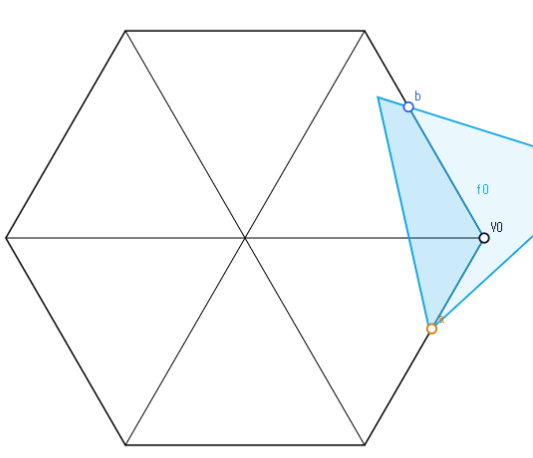
\includegraphics[width=\linewidth]
  {figures/strategy3_local_area_loss.png}
\par\smallskip
\footnotesize (a) local retained area
\end{minipage}\hfill
\begin{minipage}[b]{.48\textwidth}
\centering
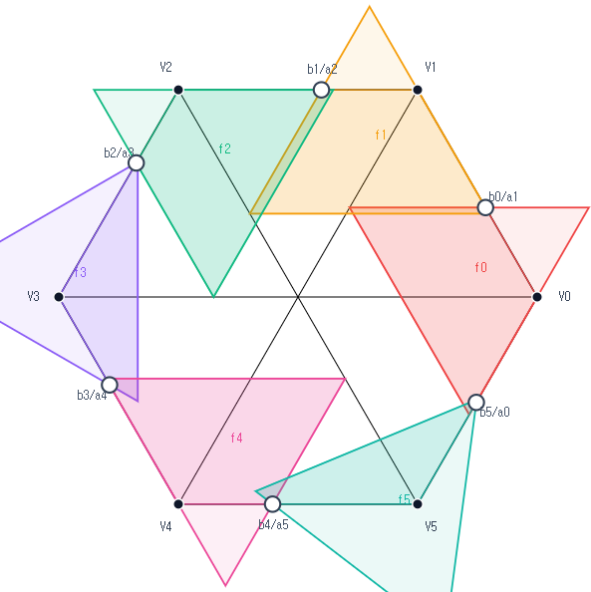
\includegraphics[width=\linewidth]
  {figures/strategy3_global_area_loss.png}
\par\smallskip
\footnotesize (b) cyclic retained areas
\end{minipage}
\caption{The area-loss method.  The dark regions indicate the portions
retained in $H$; the loss $\mathcal L(T)$ is the area outside $H$.}
\label{fig:area-loss}
\end{figure}

\subsection{Local area loss}

\begin{theorem}[Local square loss]
\label{thm:local-square-loss}
\label{lem:appendix-local-square-loss}

Let $T$ be a closed unit equilateral triangle containing
$V_i$, $V_i+a(V_{i-1}-V_i)$, and $V_i+b(V_{i+1}-V_i)$, where $a,b\in[0,1]$.
Then
\begin{equation}
 \mathcal L(T)\ge\min\{a,b\}^2,
 \label{eq:min-square-loss}
\end{equation}
and, if $a+b>1$,
\begin{equation}
 \mathcal L(T)\ge\max\{a,b\}^2.
 \label{eq:max-square-loss}
\end{equation}
\end{theorem}
\begin{proof}
Use the shared corner chart of \zcref{lem:shared-corner-chart} and the
orientation forms \zcref{eq:orientation-type-I,eq:orientation-type-II}.
Write $D=1-t+t^2$, $z=\sqrt D$, with $0\le t\le1$.
In Type I, containment of
$(0,0),(0,a),(b,0)$ gives
\begin{equation}
 \alpha\ge tb,\quad \beta\ge(1-t)a,
 \quad \alpha+\beta+(1-t)b\le z,
 \quad \alpha+\beta+ta\le z.                 \label{eq:area-type-I-containment}
\end{equation}
The two inequalities defining $W$ become
\[
 (1-t)U+V\ge(1-t)\alpha+\beta,
 \qquad U+tV\ge\alpha+t\beta.
\]
For fixed $t$, lowering $\alpha$ or $\beta$ therefore enlarges $T\cap W$.
The outside loss is minimized at
$\alpha=tb$, $\beta=(1-t)a$.  At that placement the portion outside $W$
has vertices, in the $(U,V)$-plane,
\[
 (0,0),\quad(a+tb,0),\quad(tb,(1-t)a),
 \quad(0,b+(1-t)a).
\]
Since the Jacobian of $(x,y)\mapsto(U,V)$ has absolute value $D$,
\begin{equation}
 \mathcal L(T)\ge \mathcal L_{\mathrm I}(a,b;t)
 =\frac{(1-t)a^2+tb^2+2t(1-t)ab}{D}.          \label{eq:type-I-loss}
\end{equation}
If $a\le b$, then
\[
 D(\mathcal L_{\mathrm I}-a^2)
 =t\{b^2-a^2+(1-t)(a^2+2ab)\}\ge0;
\]
the reflected factorization proves $\mathcal L_{\mathrm I}\ge b^2$ when $b\le a$.
This proves \eqref{eq:min-square-loss} in Type I.

Suppose now that $a+b>1$ and $a\le b$.  Set
\[
 r=\frac ab,\qquad t_0=\frac{1-r^2}{1+2r}.
\]
Since $b>1/(1+r)$, feasibility in \eqref{eq:type-I-loss} and
\eqref{eq:area-type-I-containment} excludes
$0\le t<t_0$: for $0<t<t_0$,
\[
 \left(\frac{1+r(1-t)}{1+r}\right)^2-D
 =\frac{t(1+2r)(t_0-t)}{(1+r)^2}>0,
\]
so $b+(1-t)a>z$, while $t=0$ would give $a+b\le1$.  Hence $t\ge t_0$, and
\[
 D(\mathcal L_{\mathrm I}-b^2)
 =(1-t)b^2\{r^2-1+t(2r+1)\}\ge0.
\]
If $b\le a$, put $r=b/a$ and
$t_1=(r^2+2r)/(1+2r)$.  The identical reflected calculation excludes
$t>t_1$ and gives
\[
 D(\mathcal L_{\mathrm I}-a^2)
 =ta^2\{r^2+2r-t(1+2r)\}\ge0.
\]
Thus \eqref{eq:max-square-loss} holds in Type I.

In Type II, substituting the axes in \zcref{eq:orientation-type-II} gives
the exact positive $y$- and $x$-axis reaches
\begin{equation}
 A=\beta,\qquad B=z-\alpha-\beta,\qquad A+B\le z\le1.
 \label{eq:area-type-II-reaches}
\end{equation}
In particular Type II is impossible when $a+b>1$.  Its wedge intersection
is the quadrilateral with vertices
\[
 (0,0),\quad(B,0),\quad
 \left(\frac{B+(1-t)A}{D},\frac{A+tB}{D}\right),
 \quad(0,A).
\]
Hence
\begin{equation}
 \mathcal L(T)=\mathcal L_{\mathrm{II}}(A,B;t)
 =1-\frac{(1-t)A^2+tB^2+2AB}{D}.              \label{eq:type-II-loss}
\end{equation}
Let $S=A+B$.  If $A\le B$, write $A=rS$, $B=(1-r)S$ with
$0\le r\le1/2$.  Since $S^2\le D$, and with
\[
 C=(1-t)r^2+t(1-r)^2+2r(1-r),
\]
we have $\mathcal L_{\mathrm{II}}\ge1-C$.  The exact factorization
\[
 1-C-r^2D=(1-t)(1-2r+tr^2)\ge0
\]
gives $\mathcal L_{\mathrm{II}}\ge r^2D\ge A^2$.  Reflection gives
$\mathcal L_{\mathrm{II}}\ge B^2$ when $B\le A$.  Since $A\ge a$ and $B\ge b$,
this proves \eqref{eq:min-square-loss}.  The two orientation types are
exhaustive, so the theorem follows.
\end{proof}

\subsection{Cyclic accumulation}

Assume here that the six V triangles cover $\partial H$, and choose
strict handoffs $\xi_i,a_i,b_i$ as in \zcref{prop:strict-handoffs}.
An \emph{ascent} at index $i$ means $\xi_{i-1}<\xi_i$, equivalently
$a_i+b_i>1$.

\begin{lemma}[Cyclic area-loss certificate]
\label{lem:cyclic-area-loss}
The six actual V triangles satisfy
\[
 \left|\{i\in\mathbb Z/6\mathbb Z:a_i+b_i>1\}\right|\ge2
 \quad\Longrightarrow\quad
 \sum_{i=0}^5\mathcal L(T_i)>1.
\]
\end{lemma}

\begin{proof}
Put $m=\min_i \xi_i$ and $M=\max_i \xi_i$.  The reflection
$y_i=1-\xi_{-i-1}$ swaps each V triangle's two coordinates and preserves the number of ascents and the total loss.  Hence assume $m\le1-M$.  Every selected
V triangle coordinate is then at least $m$, so
\eqref{eq:min-square-loss} gives loss at least $m^2$ for every V triangle.

Choose an ascent out of a minimum plateau,
$\xi_{p-1}=m<\xi_p$.  Its V triangle contains the coordinate $1-m$ and loses at least
$(1-m)^2$ by \eqref{eq:max-square-loss}.  A second ascent has one coordinate
strictly larger than $1/2$ and hence loses strictly more than $1/4$.  The
other four V triangles lose at least $m^2$ each, so the total loss is strictly
larger than
\[
 4m^2+(1-m)^2+\frac14
 =5\left(m-\frac15\right)^2+\frac{21}{20}>1.
\]

\end{proof}

\begin{proposition}[Branch closed by area]
\label{prop:area-branches}
The branch $N_{\rm gap}=0$, $N_+\ge2$ is impossible.
\end{proposition}
\begin{proof}
The six V triangles cover $\partial H$. The at-least-two clause of
\zcref{prop:strict-handoffs} supplies the selection for
\zcref{lem:cyclic-area-loss}. Thus the V triangles have total normalized
inside area below five. The C triangle contributes at most one, whereas
$H$ has normalized area six. Apply \zcref{lem:open-cover-budget} with area.
\end{proof}
